\documentclass[fleqn]{article}
\oddsidemargin 0.0in
\textwidth 6.0in
\thispagestyle{empty}
\usepackage{import}
\usepackage{amsmath}
\usepackage{graphicx}
\usepackage{flexisym}
\usepackage{amssymb}
\usepackage{bigints} 
\usepackage[english]{babel}
\usepackage[utf8x]{inputenc}
\usepackage{float}
\usepackage[colorinlistoftodos]{todonotes}

\definecolor{hwColor}{HTML}{AD53BA}

\begin{document}

  \begin{titlepage}

    \newcommand{\HRule}{\rule{\linewidth}{0.5mm}} % Defines a new command for the horizontal lines, change thickness here

    \center % Center everything on the page



    \textsc{\LARGE Arizona State University}\\[1.5cm] % Name of your university/college

    \textsc{\LARGE Mathematical Methods For Physics II }\\[1.5cm] % Major heading such as course name


    \begin{figure}
      
\includegraphics[width=\linewidth]{asu.png}
    \end{figure}


    \HRule \\[0.4cm]
    { \huge \bfseries Homework Ten}\\[0.4cm] 
    \HRule \\[1.5cm]

    \textbf{Behnam Amiri}

    \bigbreak

    \textbf{Prof: Cecilia Lunardini}

    \bigbreak


    \textbf{{\large \today}\\[2cm]}

    \vfill % Fill the rest of the page with whitespace

  \end{titlepage}

  \textbf{Part A}
  \begin{enumerate}

    \item Expand the generating function of the Legendre Polynomials to derive the first three Legendre Polynomials. 
    (Hint: It is probably easiest here to compute the first three terms in the Taylor's series expansion. One could also use the binomial expansion for  $[1 -( 2hx - h^2 ) ]^{-1/2}$, but keeping track of the terms would be more complicated.)

      \textcolor{hwColor}{
        Page 584 of the text book states that the generating function is 
        $$G(x,h)=\left(1-2xh+h^2\right)^{-1/2}=\sum\limits_{n=0}^{\infty} P_n(x) h^n$$
        \\
        \textbf{A quick review:} \\
        \\
        We learned about the Taylor series in our primary calculus classes which is \emph{(It is a series that is used to create an estimate (guess) of what a function looks like)}
        $$\sum\limits_{n=0}^{\infty} \dfrac{f^{(n) (a)}}{n!}(x-a)^n$$
        \\
        \\
        So let's take the Taylor series with respect to h
        \\
        \\
        $
          \sum\limits_{n=0}^{2} \dfrac{G^n(h)}{n!} y^n=\dfrac{G(h)y^0}{0!}+\dfrac{G^'(h)y}{1!}+\dfrac{G^{''}(h)y^2}{2!} \\
          \\
          \\
          =\dfrac{\left(1-2xh+h^2\right)^{-1/2} y^0}{0!}
          +\dfrac{-\dfrac{1}{2}(-2x+2h)(1-2xh+h^2)^{-\dfrac{3}{2}}}{1!} \\
          \\
          +\dfrac{-\dfrac{1}{2} \left[2(1-2xh+h^2)^{-\dfrac{3}{2}}+(-2x+2h)(-\dfrac{3}{2})(-2x+2h)(1-2xh+h^2)^{-\dfrac{5}{2}}\right]}{2!}
        $ 
        \\
        \\
        \\
        Evaluate at $h=0$: \\
        \\
        \\
        $
          \sum\limits_{n=0}^{2} \dfrac{G^n(0)}{n!} y^n=y^0+xy+\dfrac{y^2(3x^2-1)}{2} \\
          \\
          \\
          \\
          \therefore ~~~ \begin{cases}
            P_0(x)=1 \\
            \\
            P_1(x)=x \\
            \\
            P_2(x)=\dfrac{3x^2-1}{2}
          \end{cases}
        $
      }

    \item  Show that the generating function in Eq. 18.15 of the textbook is consistent with Legendre's equation.
    (Hint: Take the appropriate first and second derivatives of both sides of Eq. 18.15 (middle and right expressions), and arrange a combination of the left-hand-side results that will vanish.  You should get to a point where it becomes clear that the $P_l(x)$ that appear in Eq. 18.15 indeed satisfy Legendre equation.)

      \textcolor{hwColor}{
        From the textbook we have equation 18.15 as: 
        $$G(x,h)=\left(1-2xh+h^2\right)^{-\dfrac{1}{2}}=\sum\limits_{n=0}^{\infty} P_n(x) h^n$$
        This equation is valid for $|h|<1$ and $|x|<1$. The function on the left is called the generating function for the 
        Legendre polynomials because all of them appear as the coefficients in the power series expansion. To prove the
        above equation, we note the left side is an analytic function of $x$ for $|x|<1$, which means that it has a power series expansion.
        $$G(x,h)=\sum\limits_{n=0}^{\infty} Q_n(h) h^n$$
        Explicit differentiation of $G(x,h)$ shows that it satisfies the PDE 
        $$\left[G_x(1-x^2)\right]_x+x\left[xG\right]_{xx}=0$$
        Plugging the expansion into this PDE, we find that \\
        $$\sum\limits_{n=0}^{\infty} \left[\left(1-z^2\right) Q^'_n(x) \right]^' t^n+\sum\limits_{n=0}^{\infty} n \left(n+1\right) Q_n(x) h^n=0$$
        Because the coefficients must match, we must have
        $$\left[\left(1-x^2\right) Q^'_n(x) \right]^'+n \left(n+1\right) Q_n(x)=0$$
        So $Q_n$ satisfies Legendre’s differential equation! \\
        \\
        On the other hand, putting $z=1$ in the definition of $G(x,h)$, we have
        $$G(1,h)=\left(1-2h+h^2\right)^{-1/2}=\left(1-h\right)^{-1}=\sum\limits_{n=0}^{\infty} h^n$$
        so that $Q_n(1)=1$. This determines which solution of Legendre’s equation $Q_n$ is, namely $Q_n \equiv P_n$. 
        This proves $G(x,h)=\left(1-2xh+h^2\right)^{-\dfrac{1}{2}}=\sum\limits_{n=0}^{\infty} P_n(x) h^n$.
        \\
        \\
        \rule{15cm}{1pt}
        \\
        \\
        Another way to approach this problem is \\
        \\
        $G(x,h)=\left(1-2xh+h^2\right)^{-\dfrac{1}{2}}=\sum\limits_{n=0}^{\infty} P_n(x) h^n \\$
        \\
        \\
        \textbf{L.H.S:} \\ \\
        $
        \begin{cases}
          \dfrac{\partial G}{\partial x}=h\left(1-2xh+h^2\right)^{-3/2} \\
          \\
          \dfrac{\partial G}{\partial h}=\left(x-h\right)\left(1-2xh+h^2\right)^{-3/2}
        \end{cases}
        $ \\
        \\
        \\
        \textbf{R.H.S:} \\ \\
        $
          \begin{cases}
            \dfrac{\partial G}{\partial x}=\sum\limits_{n=0}^{\infty} P^'_n h^n \\
            \\
            \dfrac{\partial G}{\partial h}=\sum\limits_{n=0}^{\infty} n P_n h^{n-1} h^'
          \end{cases} \\
          \\
          \\
          \\
          \Longrightarrow \dfrac{\partial G}{\partial x}=h\left(1-2xh+h^2\right)^{-3/2}=\sum\limits_{n=0}^{\infty} P^'_n h^n \\
          \\
          \\
          h \left(1-2xh+h^2\right)^{-1/2} \left(1-2xh+h^2\right)^{-1}=\sum\limits_{n=0}^{\infty} P^'_n h^n \\
          \\
          \\
          h \sum\limits_{n=0}^{\infty} P_n(x) h^n=\left(1-2xh+h^2\right) \sum\limits_{n=0}^{\infty} P^'_n h^n \\
          \\
          \\
          \therefore ~~~ \sum\limits_{n=0}^{\infty} P_n h^n= \sum\limits_{n=0}^{\infty} P^'_n h^{n-1}-2x \sum\limits_{n=0}^{\infty} P^'_n h^n+\sum\limits_{n=0}^{\infty} P^'_n h^{n+1} ~~~~~ \mathbf{(A)} \\ \\
          \\
        $
          Dividing $\dfrac{\partial G}{\partial h}$ by $\dfrac{\partial G}{\partial x}$: \\
          \\
          \\
          $
            \dfrac{\left(x-h\right)\left(1-2xh+h^2\right)^{-3/2}=\sum\limits_{n=0}^{\infty} n P_n h^{n-1} h^'}{h\left(1-2xh+h^2\right)^{-3/2}=\sum\limits_{n=0}^{\infty} P^'_n h^n} \\
            \\
            \\
            \Longrightarrow \left(x-h\right) \sum\limits_{n=0}^{\infty} P^'_n h^n=h \sum\limits_{n=0}^{\infty}n P_n h^{n-1} 
            \Longrightarrow x \sum\limits_{n=0}^{\infty}P^'_n h^n-\sum\limits_{n=0}^{\infty}P^'_n n h^{n+1} =\sum\limits_{n=0}^{\infty} n P_n h^n ~~~~~ \mathbf{(B)} \\
            \\
            \\
            \\
            \mathbf{(A)}-\mathbf{(B)}= 
            \left[-\sum\limits_{n=0}^{\infty} P_n h^n+\sum\limits_{n=0}^{\infty} P^'_n h^{n-1}-2x \sum\limits_{n=0}^{\infty} P^'_n h^n+\sum\limits_{n=0}^{\infty} P^'_n h^{n+1}\right]
            -
            \left[x \sum\limits_{n=0}^{\infty}P^'_n h^n-\sum\limits_{n=0}^{\infty}P^'_n n h^{n+1}-\sum\limits_{n=0}^{\infty} n P_n h^n\right]
            \\
            \\
            \\
            \\
            \Longrightarrow \left[P_n-P^'_{n+1}+2xP^'_n-P^'_{n-1}\right]-\left[xP^'_n-P^'_{n-1}-nP^'_n\right]=P_n-P^'_{n+1}+xP^'_n+nP_n=0 \\
            \\
            \\
            \therefore ~~~ P_n(1+n)=P^'_{n+1}-xP^'_n ~~~ \surd
          $ \\
          \\
          \\
          Setting $n$ to $n-1$: \\
          \\
          \\
          $
            \left(n P_{n-1}-P^'_n+xP^'_{n-1}\right)+\left(x^2 P^'_n-xP^'_{n-1}-xnP_n\right) \\
            \\
            \\
            \\
            \therefore ~~~ (1-x^2)P^'_n-n(P_{n-1}-xP_n)=0 ~~~ \surd
            \\
            \\
            \\
            \dfrac{\partial}{\partial x}\left[(1-x^2)P^'_n-n(P_{n-1}-xP_n)\right]
            =\left[(1-x^2)P^{''}_n-2xP^'_n\right]
            +n\left[\left(P^'_{n-1}-xP^'_n\right)-P_n\right] \\
            \\
            \\
            \\
            \therefore ~~~ (1-x^2)P^{''}_n-2xP^'_n+n P_n(1+n)=0 ~~~ \surd
          $
          \\
          \\
          What we found statisfies the legendre’s differential equation. $(1-x^2)y^{''}-2xy^'+\ell (\ell+1)y=0$
      }

    \item The Legendre Polynomials enter quite naturally into expressions for the electrical or gravitational potentials of
    point sources through the inverse distance factor,
    \begin{equation}
    \frac{1}{| {\mathbf r}_s -{\mathbf r}_f |}
    \end{equation}

    Let $x$ be the cosine of the angle between ${\mathbf r}_s$ and ${\mathbf r}_f$ , and show that
    \begin{equation}
    \frac{1}{| {\mathbf r}_s -{\mathbf r}_f |} = \frac{1}{r_{>}} \sum^{\infty}_{n=0} \left( \frac{r_{<}}{r_{>}}\right)^n P_n(x)
    \end{equation}
    where $r_{<}$ ($ r_{>}$ ) is the lesser (greater) of $|{\mathbf r}_s|$ and $|{\mathbf r}_f|$.

    (Hint: Write $| {\mathbf r}_s -{\mathbf r}_f |$ as $\sqrt{({\mathbf r}_s -{\mathbf r}_f )\cdot ({\mathbf r}_s -{\mathbf r}_f )}=\sqrt{|{\mathbf r}_s|^2 +|{\mathbf r}_f |^2 -2 {\mathbf r}_s \cdot {\mathbf r}_f }$ and compare with eq. 18.15. Apply convergence requirements in order to assign the  $r_{<}$ and  $ r_{>}$ notation) 

    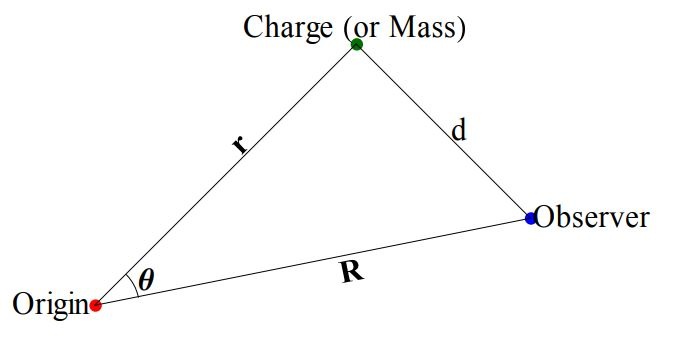
\includegraphics[height=6cm, width=15cm]{legendre.JPG}
    \textcolor{hwColor}{
      A particular use of the generating function Eq. 18.15 is in representing the inverse distance between two points 
      in three-dimensional space in terms of Legendre polynomials. The above figure shows a particle at the head of vector 
      $\mathbf{r}$ with respect to a fixed origin. An observer is located at the end of the vector denoted as $\mathbf{R}$. 
      Quite often in physics, we want to describe the potential field measured at R generated by the particle located 
      at $\mathbf{r}$. In this case it does not matter if we are interested in the potential arising from an electric or
      gravitational field of the particle; since both fields follow inverse square laws, their
      potentials are expressible in the same mathematical format. 
      \\
      \\
      We know that the the potential of a $\dfrac{l}{r^2}$ field goes as $\dfrac{l}{r}$ so that the
      potential of the particle at the observer will go as $\dfrac{K}{d}$, where $K$ is some constant and $d$ is 
      the magnitude of the vector $\mathbf{d}$. \\
      \\
      By expressing the potential at the observer in terms of the coordinate system in which the origin is at $(0,0,0)$, 
      we need to write $\mathbf{d}$ in terms of $\mathbf{r}$, $\mathbf{R}$ and $\mathbf{\theta}$. The law of cosines says: \\
      \\
      \\
      $$d^2=r^2+R^2-2rR cos(\theta) \Rightarrow d=\left(r^2+R^2-2rR cos(\theta)\right)^{1/2}$$ \\
      The key here is that we assume $R>r$. \\
      $$d=R\left(1+\left(\dfrac{r}{R}\right)^2-2 \left(\dfrac{r}{R}\right) cos(\theta)\right)^{1/2}$$
      let's set $h=\dfrac{r}{R}$ and as we are told $x=cos(\theta)$, hence: \\
      \\
      $$d=R\left(1+h^2-2hx\right)^{1/2}$$
      Now we can write the potential measured by the observer as: \\
      \\
      $$V=\dfrac{K}{d}=\dfrac{K}{\sqrt{1+h^2-2hxs}}$$
      Time to take the power series expansion for the above expression. For simplicity, we shall assume
      $\dfrac{1}{\sqrt{1-y}}$ where $y=2hx-h^2$. The power expansion is: \\
      \\
      $
        \dfrac{1}{\sqrt{1-y}}=f(0)+f^'(0)y+\dfrac{f^{''}(x) y^2}{2!}+\dfrac{f^{'''}(3!)}{y^3}+...
      $
      \\
      \\
      Taking the derivative, \\
      \\
      $
        f(y)=\dfrac{1}{\sqrt{1-y}}=1+\dfrac{y}{2}+\dfrac{1}{2} \dfrac{3}{2} \dfrac{y^2}{2!}+\dfrac{1}{2} \dfrac{3}{2} \dfrac{5}{2} \dfrac{y^3}{3!}+... \\
        \\
        =1+\dfrac{y}{2}+\dfrac{3y^2}{8}+\dfrac{5y^3}{16}+\dfrac{35y^4}{128}+...
      $ \\
      \\
      \\
      Setting $y=2hx-h^2$ we have: \\
      \\
      $
        \dfrac{1}{\sqrt{1-y}}=\dfrac{1}{\sqrt{1-2hx+h^2}}=\dfrac{2hx-h^2}{2}+\dfrac{3(2hx-h^2)^2}{8}+\dfrac{5(2hx-h^2)^3}{16}+\dfrac{35(2hx-h^2)^4}{128}+... \\
        \\
        \\
        =1+hx-\dfrac{h^2}{2}+\dfrac{3(hx)^2}{2}-\dfrac{3h^3 x}{2}+\dfrac{3h^4}{8}+\dfrac{5(hx)^3}{2}-\dfrac{15 h^4 x^2}{4}+\dfrac{15h^5 x}{8}-\dfrac{5h^6}{16}+... \\
        \\
        \\
        \Longrightarrow \dfrac{1}{\sqrt{1-y}}=\dfrac{1}{\sqrt{1-2hx+h^2}}=1+hx+\left(\dfrac{3x^2}{2}-\dfrac{1}{2}\right)h^2+\left(\dfrac{5x^3}{2}-\dfrac{3x}{2}\right)h^3+... \\
        \\
      $
      Now what we just found is a power series in powers of $h$. \\
      \\
      \\
      We recognize each coefficient as the Legendre Polynomial of order , so that we can write our series expansion as: \\
      \\
      \\
      $
        \dfrac{1}{\sqrt{1+h^2-2hx}}=P_0(x)+P_1(x)h+P_2(x)h^2+P_3(x) h^3+... \\
        \\
        \\
        \therefore ~~~ \dfrac{1}{\sqrt{1+h^2-2hx}}=\sum\limits_{\ell=0}^{\infty} P_{\ell}(x) h^{\ell} ~~~ \surd
      $ \\
      \\
      \\
      This is a very important relationship, because it allows us to write Legendre functions in
      terms of the power expansion of a well known function. We define: \\
      \\
      $$G(x,h)=\dfrac{1}{\sqrt{1+h^2-2hx}}=\sum\limits_{\ell=0}^{\infty} P_{\ell}(x) h^{\ell}$$
      for values of $|h|<1$. This is infact, what we had in the previous problem as the 
      \emph{\textbf{generating function for Legendre polynomials}} because we can
      generate Legendre Polynomials by expanding $G(x,h)$ as a power series. \\
      \\
      we can look back at our expression for potential observed at the location $\mathbf{R}$ in terms
      of Legendre polynomials as
      $$V=\dfrac{K}{d}=\dfrac{K}{R\sqrt{1+h^2-2hx}}=\dfrac{K}{R} \sum\limits_{\ell=0}^{\infty} P_{\ell}(x) h^{\ell} ~~~~~ \surd$$
    }

  \end{enumerate}

  \pagebreak

  \textbf{Part B}
  \begin{enumerate}
    \item Show that, if $P_l(x)$ is the Legendre Polynomial of order $l$, then $P^m_l(x)$  as given in Eq. 18.32 of the textbook satisfies
    the associated Legendre equation. (Hint:  Substitute directly into the associated Legendre equation, and use the product rule of differentiation. Then differentiate Legendre's equation $m$ times and compare). 

      \textcolor{hwColor}{
        From the textbook we have equation 18.32 as: 
        $$P^m_{\ell}=(1-x^2)^{m/2} \dfrac{d^m P_{\ell}}{dx^m}$$
        Also from the textbook, the associated Legendre (Equation 18.28) is 
        $$(1-x^2)y^{''}-2xy^'+\left[\ell (\ell+1)-\dfrac{m^2}{1-x^2}\right]y=0$$
        \\
        \\
        Rewriting 18.28: \\
        \\
        $
          (1-x^2)P^{''}_{\ell}-2xP^'_{\ell}+\left[\ell (\ell+1)-\dfrac{m^2}{1-x^2}\right]y=0 ~~~~~ \mathbf{(A)} \\
          \\
          \\
          \begin{cases}
            w=1-x^2 \\
            \\
            k=\dfrac{m}{2}
          \end{cases} \Rightarrow P_{\ell}=q^n \mu \\
          \\
          \\
          \dfrac{d P_{\ell}}{dx}=\mu (q^n)^'+q^n \mu^'=g^n \mu^'-mx\mu q^{n-1} ~~~ \surd
          \\
          \\
          \\
          \dfrac{d^2 P_{\ell}}{dx^2}=\dfrac{d}{dx} \left[\dfrac{d P_{\ell}}{dx}\right]=\dfrac{d}{dx}\left[g^n \mu^'-mx\mu q^{n-1} \right] \\
          \\
          \\
          =\left[-mx q^{n-1} \mu^' +q^n \mu^{''}\right]-\left[ (mx)^' q^{n-1} \mu +mx \mu(q^{n-1})^' - mx \mu ^'q^{n-1} \right] \\
          \\
          \\
          =-mx \mu^' q^{n-1}+q^n \mu^{''}-mx \mu q^{n-1}+2mx^2 \mu \left(\dfrac{m}{2}-1\right) q^{n-1}-mx \mu^' q^{n-1}
        $
        Doing a bit of algebra we have: \\
        \\
        \\
        $
          \therefore ~~~ \dfrac{d^2 P_{\ell}}{dx^2}=q^n \left[-2mxq^{-1} \mu^' -m q^{-1} \mu +\mu^{''}-2mx^2 q^{-2} \mu+m^2 x^2 q^{-2} \mu\right] \\ \\
        $
        \\
        \\
        We can rewrite \textbf{(A)} as (set be the coefficient of $P_{\ell}$ as $\gamma$)
        \\
        \\
        $q P^{''}-2xP^'+ \gamma P=0  ~~~~~ \mathbf{(B)}$ \\
        \\
        \\
        Now that we have both $\dfrac{d P_{\ell}}{dx}$ and $\dfrac{d^2 P_{\ell}}{dx^2}$, we can plug them into \textbf{(B)}.
        \\
        \\
        $
          q q^n \left[-2mxq^{-1} \mu^' -m q^{-1} \mu +\mu^{''}-2mx^2 q^{-2} \mu+m^2 x^2 q^{-2} \mu\right] \\ 
          -2x \left[g^n \mu^'-mx\mu q^{n-1}\right]+\gamma q^n \mu=0 
          \\
          \\
          \\
          q^n \left[q \mu^{''}-2mx \mu^' -m \mu-2mx^2 q^{-1} \mu+m^2 x^2 q^{-1} \mu \right]-2x \left[g^n \mu^'-mx\mu q^{n-1}\right]+\gamma q^n \mu=0 \\
          \\
          \\
          q \mu^{''}-2mx \mu^'-m \mu-2mx^2 q^{-1} \mu+m^2 x^2 q^{-1} \mu-2x \mu^'+2mx^2 q^{-1} \mu+\gamma \mu=0 \\
          \\
          \\
          \mu^{''} q-2x \mu^' (m+1)+(m^2 x^2 q^{-1}-m+\gamma) \mu=0 
          \\
          \\
          \\
          \mu^{''} q-2x \mu^' (m+1)+\left[-m^2 q^{-1} (1-x^2)-m+\ell(\ell+1)\right] \mu=0 \\
          \\
          \\
          \\
          \therefore ~~~ q \mu^{''}-2x(m+1) \mu^'+\left[(\ell-m)(\ell++1)\right] \mu=0 ~~~ \surd
        $
        \\
        \\
        \\
        What we just found is has the same format as the \textbf{\emph{Then differentiateLegendre’s equationmtimes and compare}}. 
      }

    \item Show, using Eq. 18.33, that
    $Y^{-m}_l (\theta, \phi) = (-1)^m Y^{m\ast }_l (\theta, \phi) $, 
    where $Y^{-m}_l (\theta, \phi)$ is the complex conjugate of $Y^{m\ast }_l (\theta, \phi)$.

      \textcolor{hwColor}{
        From the textbook we have equation 18.33 as:
        $$P^{-m}_{\ell}(x)=(-1)^m \dfrac{(\ell-m)!}{(\ell+m)!} P^m_{\ell}(x)$$ 
        \\
        \\
        \\
        The spherical harmonics $Y^m_{\ell}(\theta,\phi)$ are defined as
        $$
          Y^m_{\ell}(\theta,\phi)=(-1)^m \left[ \dfrac{2\ell+1}{4\pi} \dfrac{(\ell-m)!}{(\ell+m)!} \right]^{\dfrac{1}{2}} P^m_{\ell} ~ cos\theta ~ exp(im \phi)
        $$ 
        \\
        \\
        \\
        $
          Y^{-m}_{\ell}(\theta,\phi)=(-1)^m \left[ \dfrac{2\ell+1}{4\pi} \dfrac{(\ell+m)!}{(\ell-m)!} \right]^{\dfrac{1}{2}} \left[(-1)^m \dfrac{(\ell-m)!}{(\ell+m)!} P^m_{\ell}(x)\right] ~ cos\theta ~ exp(-im \phi) \\
          \\
          \\
          =(-1)^m (-1)^m \left[ \dfrac{2\ell+1}{4\pi} \dfrac{(\ell+m)!}{(\ell-m)!} \dfrac{\left[(\ell-m)!\right]^2}{\left[(\ell+m)!\right]^2} \right]^{\dfrac{1}{2}}  P^m_{\ell}(x) ~ cos\theta ~ exp(-im \phi) \\
          \\
          \\
          =(-1)^m (-1)^m \left[ \dfrac{2\ell+1}{4\pi} \dfrac{(\ell-m)!}{(\ell+m)!} \right]^{\dfrac{1}{2}}  P^m_{\ell}(x) ~ cos\theta ~ exp(-im \phi) \\
          \\
          \\
          \\
          \therefore ~~~ Y^{-m}_{\ell}(\theta,\phi)=(-1)^m Y^{m \ast}_{\ell}(\theta,\phi) ~~~ \surd
        $
      }

  \end{enumerate}

\end{document}
